\documentclass[12pt]{article}
% Geometria i fonty odtworzone z sprawozdanie_wzor.pdf: letterpaper 612x792 pt,
% szerokosc tekstu 390 pt, fonty CMR12 - czyli domyslne ustawienia klasy article
% w rozmiarze 12pt, bez pakietu geometry.
\usepackage{iftex}
\ifPDFTeX
  \usepackage[utf8]{inputenc}
\else
  % galaz dla xelatex/tectonic: ten sam dokument sklada sie obiema drogami
  \usepackage{fontspec}
  \setmainfont{lmroman10-regular.otf}[
    BoldFont       = lmroman10-bold.otf,
    ItalicFont     = lmroman10-italic.otf,
    BoldItalicFont = lmroman10-bolditalic.otf]
\fi
\usepackage[polish]{babel}
\usepackage{amsmath,amssymb}
\usepackage{booktabs}
\usepackage{graphicx}
\usepackage{caption}
% babel ustawia \refname dopiero przy \begin{document}
\addto\captionspolish{\renewcommand{\refname}{Bibliografia}}

\title{\textbf{Zadanie nr 1 - trening neuronu liniowego}\\[2mm]
       \large Inteligentna Analiza Danych}
\author{Łukasz Centkowski 264303 \\ Maciej Dominiak 264307}
\date{25 października 2026}

\begin{document}
\maketitle
\thispagestyle{empty}
\newpage

\section{Cel zadania}

Celem zadania było ustalenie, od czego zależy jednoznaczność wag końcowych
neuronu liniowego trenowanego wieloma wzorcami oraz czy skuteczny trening jest
w~ogóle osiągalny. Oba pytania badano w~trzech konfiguracjach różniących się
relacją liczby wag~$N$ do liczby wzorców~$M$, a~uzyskane obserwacje zinterpretowano
przez pryzmat równoważności treningu z~zadaniem rozwiązywania układu równań
liniowych.

\section{Wstęp teoretyczny}

Trening neuronu liniowego regułą delty jest gradientową minimalizacją błędu
średniokwadratowego~\cite{widrow}. Ponieważ wyjście neuronu zależy od wag liniowo,
żądanie zerowego błędu na wszystkich wzorcach sprowadza się do układu równań
\begin{equation}
\mathbf{X}\mathbf{w} = \mathbf{t}, \qquad \mathbf{X} \in \mathbb{R}^{M \times N},
\end{equation}
gdzie wierszami $\mathbf{X}$ są wzorce treningowe, a~wagi pełnią rolę
niewiadomych~\cite{wyklad}. Liczba wzorców to liczba równań, liczba wag to liczba
niewiadomych.

Każda poprawka wag jest wielokrotnością prezentowanego wzorca, więc przyrost
$\mathbf{w}-\mathbf{w}_0$ leży w~przestrzeni wierszowej $\mathbf{X}$, a~składowa
z~jądra tej macierzy zostaje taka, jaka wypadła w~losowaniu. Granicą treningu jest
\begin{equation}
\mathbf{w}_\infty = \mathbf{w}_0 + \mathbf{X}^{+}\left(\mathbf{t} - \mathbf{X}\mathbf{w}_0\right),
\label{eq:granica}
\end{equation}
gdzie $\mathbf{X}^{+}$ jest pseudoodwrotnością $\mathbf{X}$. Wpływ wag początkowych
zależy więc od wymiaru jądra, czyli od rzędu macierzy~\cite{osowski}. Krok uczący przyjęto jako $\eta = 0{,}1$, wspólny dla wszystkich eksperymentów.
Przy stałym kroku reguła przyrostowa nie zatrzymuje się dokładnie w~punkcie
granicznym, lecz w~jego otoczeniu o~promieniu rzędu $\eta$~\cite{widrow}; obciążenie
to jest widoczne w~wynikach jako niewielka odchyłka od wartości
przewidzianej~(\ref{eq:granica}).

\section{Eksperymenty i wyniki}

We wszystkich eksperymentach stosowano przyrostową regułę delty: wagi poprawiano po
każdym wzorcu, a~jedynym kryterium zatrzymania była liczba epok $K=5000$. Zbiór
treningowy losowano \emph{raz} dla danej konfiguracji, a~wagi początkowe
\emph{osobno dla każdego przebiegu}, z~rozkładu jednostajnego na $[-1,1]$. Wartości
$\mathbf{X}$ i~$\mathbf{t}$ pochodzą z~rozkładu $\mathcal{N}(0,1)$, przy czym
$\mathbf{t}$ losowano niezależnie od $\mathbf{X}$: przyjęcie
$\mathbf{t}=\mathbf{X}\mathbf{w}$ czyniłoby układ zgodnym także dla $M>N$ i~usuwało
najistotniejszy z~badanych przypadków.

\subsection{Eksperyment nr 1: układ nadokreślony \mbox{($N < M$)}}

\subsubsection{Założenia}
Neuron o~$N=3$ wagach trenowany na $M=10$ wzorcach, a~więc więcej równań niż
niewiadomych. Rząd macierzy $\mathbf{X}$ wynosi $3$, krok uczący $\eta = 0{,}1$.
Wykonano 8 przebiegów.

\subsubsection{Przebieg}
Każdy przebieg rozpoczynał się od innych wag losowych i~obejmował $K$ epok na tym
samym zbiorze treningowym. Po każdej epoce rejestrowano błąd średniokwadratowy na
całym zbiorze, wyłącznie w~celach pomiarowych.

\subsubsection{Rezultat}
Wagi końcowe wszystkich przebiegów zestawiono w~Tab.~\ref{tab:nm1}.

\begin{table}[h]
\centering
\caption{Wagi końcowe w~ośmiu przebiegach dla $N=3$, $M=10$}
\label{tab:nm1}
\begin{tabular}{ccccc}
\toprule
\textbf{Przebieg} & $w_1$ & $w_2$ & $w_3$ & \textbf{Błąd MSE} \\
\midrule
1 & 0,4185 & $-$0,2131 & $-$0,3128 & 4,962e$-$01 \\
2 & 0,4185 & $-$0,2131 & $-$0,3128 & 4,962e$-$01 \\
3 & 0,4185 & $-$0,2131 & $-$0,3128 & 4,962e$-$01 \\
4 & 0,4185 & $-$0,2131 & $-$0,3128 & 4,962e$-$01 \\
5 & 0,4185 & $-$0,2131 & $-$0,3128 & 4,962e$-$01 \\
6 & 0,4185 & $-$0,2131 & $-$0,3128 & 4,962e$-$01 \\
7 & 0,4185 & $-$0,2131 & $-$0,3128 & 4,962e$-$01 \\
8 & 0,4185 & $-$0,2131 & $-$0,3128 & 4,962e$-$01 \\
\bottomrule
\end{tabular}
\end{table}

Wagi są nieodróżnialne we wszystkich przebiegach, a~rozrzut $5{,}551\cdot10^{-17}$
leży na poziomie precyzji arytmetyki zmiennoprzecinkowej. Błąd końcowy $0{,}4962$ wobec granicy najmniejszych kwadratów $0{,}492861$
pozostawia różnicę $0{,}003$, która wynika z~omówionego wyżej obciążenia reguły
przyrostowej, a~nie z~nieskuteczności treningu.
Skuteczny trening nie był możliwy: przy losowym $\mathbf{t}$ układ dziesięciu równań
o~trzech niewiadomych jest sprzeczny, a~najlepszy kompromis jest tylko jeden.

\subsection{Eksperyment nr 2: układ kwadratowy \mbox{($N = M$)}}

\subsubsection{Założenia}
Neuron o~$N=5$ wagach i~$M=5$ wzorców, rząd macierzy $\mathbf{X}$ równy $5$, krok uczący $\eta = 0{,}1$, 8 przebiegów.

\subsubsection{Przebieg}
Jak w~eksperymencie nr~1.

\subsubsection{Rezultat}
Wyniki przedstawia Tab.~\ref{tab:nm2}.

\begin{table}[h]
\centering
\caption{Wagi końcowe w~ośmiu przebiegach dla $N=5$, $M=5$}
\label{tab:nm2}
\small
\begin{tabular}{ccccccc}
\toprule
\textbf{Przebieg} & $w_1$ & $w_2$ & $w_3$ & $w_4$ & $w_5$ & \textbf{Błąd MSE} \\
\midrule
1 & $-$1,2188 & $-$0,1165 & $-$0,2026 & 0,6470 & $-$1,4753 & 1,006e$-$29 \\
2 & $-$1,2188 & $-$0,1165 & $-$0,2026 & 0,6470 & $-$1,4753 & 1,006e$-$29 \\
3 & $-$1,2188 & $-$0,1165 & $-$0,2026 & 0,6470 & $-$1,4753 & 1,006e$-$29 \\
4 & $-$1,2188 & $-$0,1165 & $-$0,2026 & 0,6470 & $-$1,4753 & 1,006e$-$29 \\
5 & $-$1,2188 & $-$0,1165 & $-$0,2026 & 0,6470 & $-$1,4753 & 1,006e$-$29 \\
6 & $-$1,2188 & $-$0,1165 & $-$0,2026 & 0,6470 & $-$1,4753 & 1,006e$-$29 \\
7 & $-$1,2188 & $-$0,1165 & $-$0,2026 & 0,6470 & $-$1,4753 & 1,006e$-$29 \\
8 & $-$1,2188 & $-$0,1165 & $-$0,2026 & 0,6470 & $-$1,4753 & 1,006e$-$29 \\
\bottomrule
\end{tabular}
\end{table}

Wagi końcowe są nieodróżnialne, rozrzut wynosi dokładnie zero, a~błąd spada do
$1{,}0\cdot10^{-29}$. Macierz $\mathbf{X}$ jest nieosobliwa, więc układ ma dokładnie
jedno rozwiązanie i~algorytm zbiega do niego niezależnie od punktu startowego. Jest
to jedyna konfiguracja, w~której trening jest zarazem skuteczny i~jednoznaczny.

\subsection{Eksperyment nr 3: układ niedookreślony \mbox{($N > M$)}}

\subsubsection{Założenia}
Neuron o~$N=10$ wagach i~tylko $M=4$ wzorcach. Rząd macierzy $\mathbf{X}$ wynosi $4$,
więc jądro ma wymiar $10-4=6$. Krok uczący $\eta = 0{,}1$, 8 przebiegów.

\subsubsection{Przebieg}
Jak poprzednio. Dodatkowo, dla każdego przebiegu sprawdzano zgodność wag końcowych
z~granicą przewidzianą równaniem~(\ref{eq:granica}) oraz badano, czy różnice między
przebiegami leżą w~jądrze macierzy $\mathbf{X}$.

\subsubsection{Rezultat}
Wagi końcowe zestawiono w~Tab.~\ref{tab:nm3}; ze względu na liczbę wag tabelę podano
w~układzie transponowanym.

\begin{table}[h]
\centering
\caption{Wagi końcowe w~ośmiu przebiegach dla $N=10$, $M=4$}
\label{tab:nm3}
\footnotesize
\begin{tabular}{lrrrrrrrr}
\toprule
 & \multicolumn{8}{c}{\textbf{Przebieg}} \\
\cmidrule(l){2-9}
\textbf{Waga} & 1 & 2 & 3 & 4 & 5 & 6 & 7 & 8 \\
\midrule
$w_1$    & $-$1,148 & $-$0,932 & $-$0,322 & $-$0,932 & $-$0,995 & $-$0,444 & $-$0,359 & $-$1,289 \\
$w_2$    &    0,232 &    0,688 &    0,263 &    0,310 &    0,140 &    0,353 &    0,176 & $-$0,101 \\
$w_3$    &    0,865 & $-$0,453 &    0,213 &    0,340 &    0,735 &    0,103 &    0,847 &    0,507 \\
$w_4$    & $-$0,003 &    0,334 & $-$0,124 &    0,490 &    0,041 &    0,180 &    0,174 & $-$0,521 \\
$w_5$    & $-$0,120 &    0,579 &    0,832 &    0,652 &    0,491 &    1,079 &    1,356 &    0,569 \\
$w_6$    &    0,159 & $-$0,853 & $-$0,163 &    0,246 & $-$0,273 & $-$0,049 &    0,222 &    1,070 \\
$w_7$    &    0,428 & $-$0,315 &    0,437 &    0,668 & $-$0,350 &    0,263 & $-$0,196 & $-$0,373 \\
$w_8$    & $-$0,516 & $-$0,441 & $-$1,332 &    0,635 &    0,479 & $-$0,748 & $-$0,809 &    0,420 \\
$w_9$    & $-$0,303 &    0,777 &    0,312 &    0,337 &    0,697 &    0,467 &    0,295 &    0,591 \\
$w_{10}$ & $-$0,423 &    0,317 &    0,071 & $-$0,625 & $-$1,196 &    0,482 &    1,081 & $-$0,300 \\
\bottomrule
\end{tabular}
\end{table}

Tym razem wagi końcowe różnią się w~każdym przebiegu. Rozrzut wynosi
$2{,}276$, a~więc tyle, ile same wagi. Mimo to błąd końcowy spada do $5{,}9\cdot10^{-32}$ w~każdym przebiegu, czyli trening jest skuteczny, lecz
rozwiązanie nie jest jedyne. Zestawienie miar kontrolnych dla trzech pierwszych
eksperymentów zawiera Tab.~\ref{tab:kontrola}.

\begin{table}[h]
\centering
\caption{Miary kontrolne dla trzech badanych konfiguracji}
\label{tab:kontrola}
\small
\begin{tabular}{lccc}
\toprule
\textbf{Wielkość} & $N<M$ & $N=M$ & $N>M$ \\
\midrule
Rozrzut wag między przebiegami & 5,55e$-$17 & 0,00e$+$00 & 2,28e$+$00 \\
Błąd końcowy MSE & 4,96e$-$01 & 1,01e$-$29 & 5,93e$-$32 \\
Granica najmniejszych kwadratów       & 0,492861   & 0,000000   & 0,000000   \\
Odchyłka od granicy~(\ref{eq:granica}) & 4,40e$-$02 & 2,13e$-$14 & 2,44e$-$15 \\
$\lVert\mathbf{X}(\mathbf{w}_i-\mathbf{w}_1)\rVert$ & 8,64e$-$17 & 0,00e$+$00 & 6,11e$-$16 \\
\bottomrule
\end{tabular}
\end{table}

Najistotniejszy jest ostatni wiersz Tab.~\ref{tab:kontrola}: wagi różnią się między
przebiegami o~$2{,}276$, lecz po przemnożeniu różnic przez $\mathbf{X}$ wychodzi zero
z~dokładnością do $6\cdot10^{-16}$. Przebiegi różnią się więc wyłącznie składową
z~jądra $\mathbf{X}$, czyli w~sześciu kierunkach nieobjętych przez wzorce.

Zbieżność błędu we wszystkich trzech konfiguracjach przedstawia
Rys.~\ref{fig:zbieznosc}, a~rozrzut wag końcowych Rys.~\ref{fig:wagi}.

\begin{figure}[htbp]
\centering
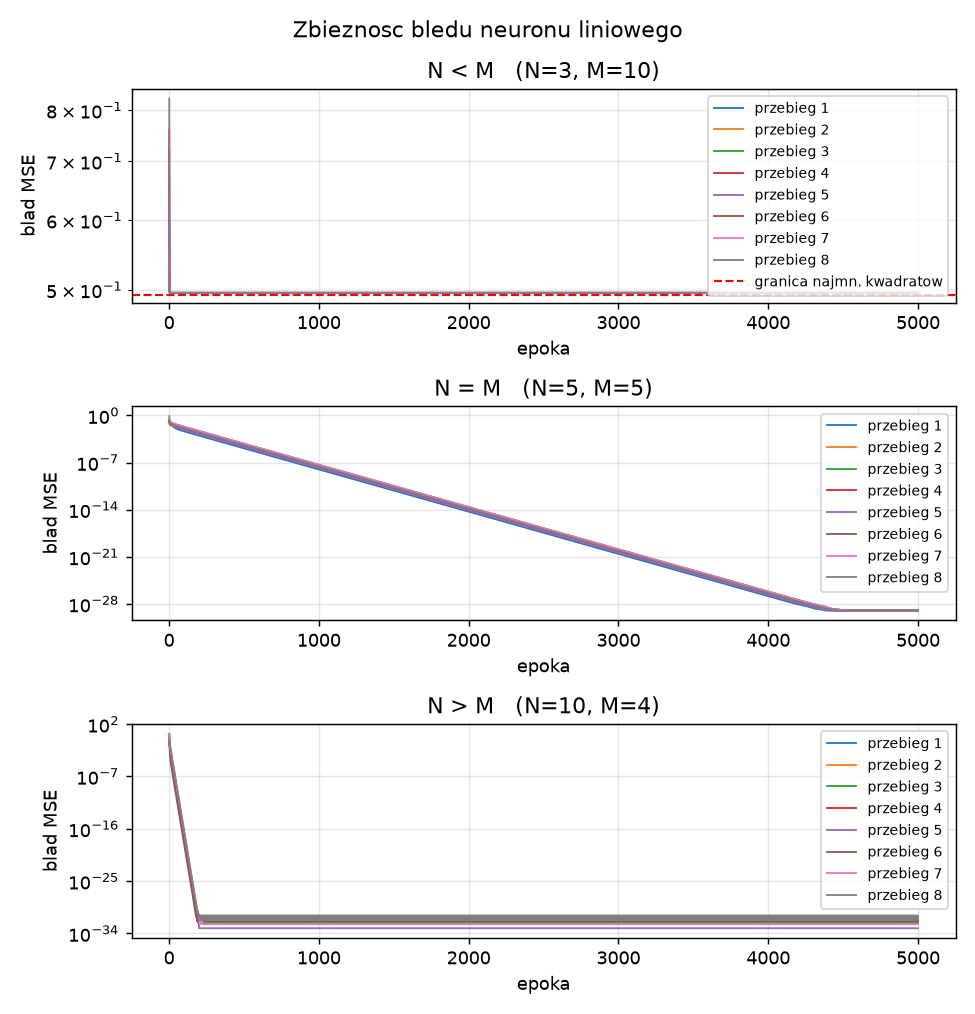
\includegraphics[width=\textwidth]{wyniki/zbieznosc_bledu.png}
\caption{Zbieżność błędu średniokwadratowego w~kolejnych przebiegach treningu}
\label{fig:zbieznosc}
\end{figure}

\begin{figure}[htbp]
\centering
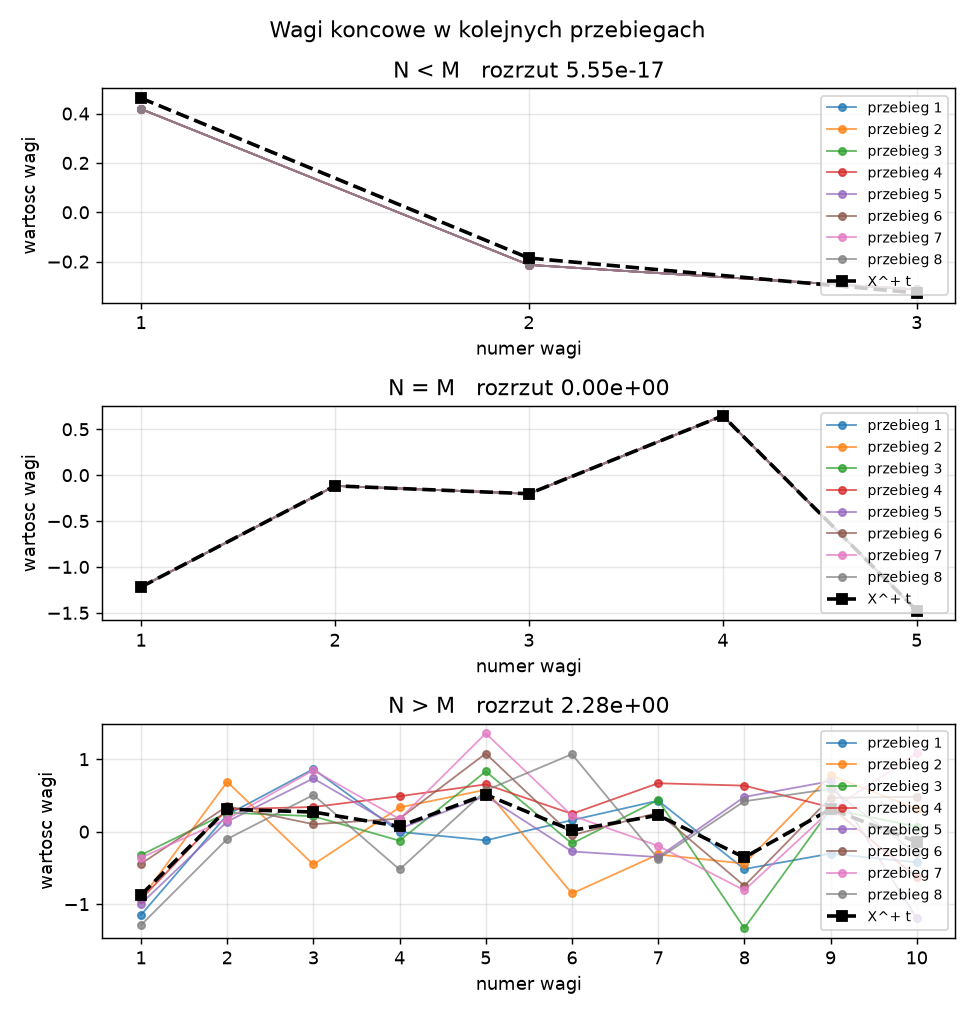
\includegraphics[width=\textwidth]{wyniki/wagi_koncowe.png}
\caption{Wagi końcowe uzyskane w~poszczególnych przebiegach na tle rozwiązania
$\mathbf{X}^{+}\mathbf{t}$}
\label{fig:wagi}
\end{figure}

Na Rys.~\ref{fig:zbieznosc} dla $N<M$ błąd osiada tuż nad granicą najmniejszych
kwadratów (linia przerywana), a~w~pozostałych konfiguracjach opada o~kilkanaście
rzędów wielkości.

Czarna przerywana linia na Rys.~\ref{fig:wagi} to najlepsze wagi
$\mathbf{X}^{+}\mathbf{t}$, wyliczone wzorem bez treningu. Dla $N<M$ i~$N=M$ neuron
dochodzi do nich (dla $N<M$ prawie), a~dla $N>M$ każdy przebieg kończy się w~innym
miejscu wokół nich.

\subsection{Eksperyment nr 4: powtarzalność dla różnych losowań zbioru}

\subsubsection{Założenia}
Jeden wylosowany zbiór treningowy nie wystarcza, aby mówić o~prawidłowości, dlatego
eksperymenty nr~1--3 powtórzono dla pięciu różnych ziaren losowania zbioru
treningowego. Dla każdego ziarna i~każdej z~trzech konfiguracji wykonano 6~przebiegów
treningu.

\subsubsection{Przebieg}
Dla ustalonego ziarna losowano zbiór $\mathbf{X}$ i~$\mathbf{t}$, a~następnie
przeprowadzano sześć przebiegów od różnych wag początkowych, dokładnie tak jak
w~eksperymentach nr~1--3. Mierzono rozrzut wag końcowych między przebiegami oraz
błąd końcowy.

\subsubsection{Rezultat}
Wyniki zestawiono w~Tab.~\ref{tab:ziarna}.

\begin{table}[h]
\centering
\caption{Rozrzut wag i~błąd końcowy dla pięciu losowań zbioru treningowego}
\label{tab:ziarna}
\small
\begin{tabular}{cccc}
\toprule
 & \multicolumn{3}{c}{\textbf{rozrzut wag / błąd MSE}} \\
\cmidrule(l){2-4}
\textbf{Ziarno} & $N<M$ & $N=M$ & $N>M$ \\
\midrule
2024  & 5,55e$-$17 / 4,96e$-$01 & 0,00e$+$00 / 1,01e$-$29 & 1,97e$+$00 / 5,01e$-$32 \\
7     & 0,00e$+$00 / 4,60e$-$01 & 0,00e$+$00 / 6,58e$-$31 & 1,90e$+$00 / 3,45e$-$32 \\
99    & 0,00e$+$00 / 8,27e$-$01 & 1,27e$-$12 / 4,93e$-$25 & 1,69e$+$00 / 3,77e$-$32 \\
12345 & 4,44e$-$16 / 7,54e$-$01 & 0,00e$+$00 / 3,71e$-$29 & 1,72e$+$00 / 8,50e$-$32 \\
555   & 8,33e$-$17 / 9,95e$-$01 & 3,55e$-$15 / 4,97e$-$30 & 1,97e$+$00 / 2,77e$-$32 \\
\bottomrule
\end{tabular}
\end{table}

Podział jest stabilny niezależnie od wylosowanego zbioru: dla $N<M$ i~$N=M$ rozrzut
wag nie przekracza $1{,}3\cdot10^{-12}$, a~dla $N>M$ mieści się między $1{,}69$
a~$1{,}97$, czyli jest tego samego rzędu co same wagi. Różnica kilkunastu rzędów
wielkości wyklucza przypadkowość obserwacji. Błąd końcowy dla $N<M$ zmienia się ze
zbiorem (od $0{,}46$ do $0{,}99$), bo zależy od stopnia sprzeczności układu, ale
nigdy nie spada do zera.

\section{Wnioski}

\paragraph{Prawidłowości w~wagach końcowych.} Są wyraźne i~skrajnie różne w~trzech
badanych konfiguracjach. Dla $N<M$ oraz $N=M$ wagi końcowe są nieodróżnialne we
wszystkich przebiegach. Rozrzut rzędu $10^{-17}$, a~dla $N=M$ dokładnie zerowy, oznacza, że punkt startowy
nie ma żadnego znaczenia. Dla $N>M$ każdy przebieg kończy się innym
zestawem wag, przy rozrzucie tego samego rzędu co same wagi. Różnice te nie są
jednak przypadkowe: leżą dokładnie w~jądrze macierzy $\mathbf{X}$, a~więc wyłącznie
w~kierunkach obojętnych dla zbioru treningowego.

\paragraph{Skuteczność treningu.} Skuteczny trening okazał się możliwy w~dwóch
z~trzech przypadków. Dla $N=M$ i~$N>M$ błąd spadł odpowiednio do $10^{-29}$ i~$10^{-32}$, czyli do zera
w~granicach precyzji obliczeń. Dla $N<M$ trening
skuteczny nie był możliwy, ponieważ błąd zatrzymał się na wartości $0{,}4962$, przy błędzie rozwiązania najmniejszych
kwadratów równym $0{,}492861$, którego z~matematycznego punktu widzenia nie da się
zmniejszyć.

\paragraph{Interpretacja.} Trening neuronu jest równoważny rozwiązywaniu
układu~(1) o~$M$ równaniach i~$N$ niewiadomych. Dla $N<M$ układ jest nadokreślony,
ponieważ równań jest więcej niż niewiadomych. Rozwiązanie dokładne nie istnieje, więc
błąd nie spada do zera. Dla $N=M$ układ ma dokładnie jedno rozwiązanie, więc wagi
końcowe są zawsze takie same. Dla $N>M$ układ jest niedookreślony, ponieważ równań
jest mniej niż niewiadomych. Rozwiązań jest nieskończenie wiele, więc każdy przebieg
kończy się innymi wagami.

\paragraph{Doprecyzowanie.} Z~równania~(\ref{eq:granica}) wynika, że o~wyniku
decyduje nie samo porównanie $N$ z~$M$, lecz rząd macierzy $\mathbf{X}$: liczba
stopni swobody pozostających neuronowi po treningu to wymiar jądra, czyli
$N - \operatorname{rank}(\mathbf{X})$. Prawidłowość można więc sformułować ogólniej:
\begin{itemize}
\item $\operatorname{rank}(\mathbf{X}) = N$ oznacza rozwiązanie jednoznaczne,
\item $\operatorname{rank}(\mathbf{X}) < N$ oznacza nieskończenie wiele rozwiązań
      zależnych od punktu startowego,
\item $\operatorname{rank}(\mathbf{X}) < M$ oznacza układ na ogół sprzeczny.
\end{itemize}

Z~praktycznego punktu widzenia najbardziej pouczający jest przypadek $N>M$: zerowy
błąd na zbiorze treningowym nie oznacza, że model został wyznaczony. Pozostaje
sześć wymiarów swobody, o~których dane nie mówią nic. Jest to ta sama sytuacja, co
przeuczenie modelu o~nadmiarowej liczbie parametrów.

\section{Załączniki}

Rdzeń implementacji, czyli pętla realizująca kroki 4--10 algorytmu treningowego
(plik \texttt{linear\_neuron.py}):

\begin{verbatim}
for k in range(epochs):                    # krok 4: dopoki k < K
    for x, z in zip(X, t):                 # kroki 5, 6, 9: mu = 1..M
        neuron.forward(x)                  # krok 7: y = w.x
        neuron.back_propagation(
            mean_squared_error_derivative(
                np.array([z]), neuron.activations[-1]))
        neuron.update_weights(learning_rate / 2.0, 0)   # krok 8
    errors[k] = float(np.mean((X @ weights(neuron) - t) ** 2))
\end{verbatim}

Krok uczący przekazywany jest jako $\eta/2$, ponieważ użyta pochodna błędu
średniokwadratowego wnosi czynnik~$2$; efektywna poprawka wag jest zatem dokładnie
równa $\eta\,(z-y)\,x_i$.

\begin{thebibliography}{9}

\bibitem{wyklad}
K. Stokfiszewski.
\textit{Inteligentna Analiza Danych. Materiały do wykładu nr 1}.
Instytut Informatyki Politechniki Łódzkiej.

\bibitem{widrow}
B. Widrow, M. E. Hoff.
\textit{Adaptive switching circuits}.
IRE WESCON Convention Record, 1960.

\bibitem{osowski}
S. Osowski.
\textit{Sieci neuronowe do przetwarzania informacji}.
Oficyna Wydawnicza Politechniki Warszawskiej, Warszawa.

\end{thebibliography}

\end{document}
